
\section{Experimental results}

\subsection{Data}

\subsubsection{Training data}

\subsubsection{Test data}\label{sec:test_data}
Mikolov \etal \cite{mikolov3} propose evaluating the regularities of the learned embedding space with a test set of analogy questions. The questions are of the form "{\it a} is to {\it b} as {\it c} is to \_\_ ". The test set contains 14 different types of analogies (see Table \ref{table:analogical}) relating to semantic concepts and grammatical relations. 

\begin{table}[h]
\small
	\caption{Analogical reasoning test set}
	\label{table:analogical}
	\centering
    \begin{tabular}{| c |  c | c |}
    \hline
    {\bf Relation} & {\bf \# Questions} & {\bf Example} \\
    \hline
     capital-common-countries & 506 & Athens : Greece \\
     & & Bangkok : Thailand\\
     \hline
    capital-world &   4524  & Abuja : Nigeria \\
    & & Accra : Ghana\\
    \hline
    currency & 866 & Algeria : dinar\\
    & & Japan : yen\\
   \hline
   city-in-state & 2467 & Chicago : Illinois \\
   & & Houston Texas\\
   \hline
    family &  506 & brother : sister \\
    & & mother : father\\
    \hline
    adjective-to-adverb & 992 & amazing : amazingly \\
    & & calm : calmly\\
    \hline
    opposite & 813 & acceptable : unacceptable \\
    & & aware : unaware\\
    \hline
    comparative & 1331 & bad : worse \\
    & & big : bigger\\
    \hline
    superlative & 1122 & bad : worst \\
    & & big : biggest\\
    \hline
    present-participle & 1056 & code : coding\\
    & & dance : dancing\\
    \hline
    nationality-adjective & 1599 & Albania : Albanian \\
    & & Argentina : Argentinean\\
    \hline
    past-tense & 1560 & dancing : danced \\
    & & decreasing : decreased\\
    \hline
    plural & 1332 & banana : bananas \\
    & & bird birds\\
    \hline
    plural-verbs &  & eat : eats \\
    & 870 & generate : generates\\
    \hline
    \end{tabular}
\end{table}


\subsection{Results}\label{sec:results}

\subsubsection{Measuring linguistic regularity via analogies}\label{results:analogy}
We evaluate the performance of (a) pre-trained Google vectors, (b) our Skip-Gram model, (c) our CBOW model, on the analogical reasoning test set introduced in section \ref{sec:test_data}. Given three query words (e.g. {\it Paris, France, London}), the task is to return the answer that fits with the analogy (in this case, {\it England}). This problem can be solved in many ways. Mikolov \etal \cite{mikolov1} propose a simple solution that relies on the inherent regularities of the embedding space learned by the Skip-Gram and CBOW models. The method uses simple vector algebra in the embedding space to find the solution word given three query words. For example, suppose the analogical relation of interest is {\it A} is to {\it B} as {\it} C is to {\it D}. Given three query words, {\it A, B, C}, the predicted solution is computed as follows:
\begin{enumerate}
\item Compute the vector representations of each word, $\phi(A), \phi(B), \phi(C)$.
\item Let $v = \phi(B) - \phi(A) + \phi(C)$.
\item Do a nearest neighbors search, based on cosine distance, to find the $k$ closest word vectors to $v$. In other words, solve for the top $k$ solutions to 
	\begin{align} \max_u 1 - \frac{ v \cdot u}{\| u \| \| v \|}\ \end{align}
\end{enumerate}

The top-$k$ accuracy is defined as the number of times $D$ appears in the set of $k$ closest words to $v$. The intuition behind this method is that the cosine distance between $\phi(A - B)$ and $\phi(C - D)$ is small when {\it A} and {\it B} are analogous to {\it C} and {\it D}. Figure \ref{fig:offsets} illustrates this intuition. 

\begin{figure}[h]
\centering
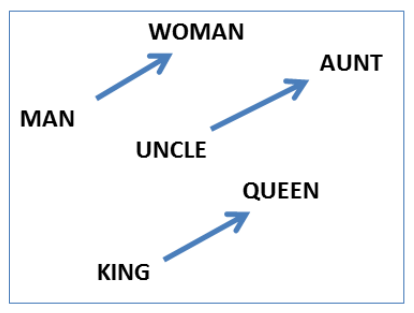
\includegraphics[width=.45\textwidth]{./images/king_queen.png}
\caption{Vector offsets for three analogous word pairs.}
\label{fig:offsets}
\end{figure}

Table \ref{tab:analogical_acc} shows the top-$k$ accuracy on the analogical reasoning dataset of the pre-trained Google vectors (GoogleVec) and the Skip-Gram and CBOW models that we trained. The Google vectors outperform both of our trained models for all $k$. This is to be expected since the Google vectors were trained on far more data than we have access to. 

Our CBOW model performs consistently worse than our Skip-Gram model. We hypothesize that this is a factor of the amount of training data we used to train our models. The CBOW model throws away a lot of information by ignoring the ordering of words. In the limit of infinite data, the bag-of-words assumption might not matter, however in a limited data setting we believe the CBOW model is hurt more than the Skip-Gram model due to the loss of information. 

Figure \ref{fig:top_k} plots the top-$k$ accuracy as a function of $k$ for the three models split up by analogy types. Figure \ref{fig:accuracy_per_question}  plots the top-5 accuracy of the three models for each of the analogy question types. A very interesting pattern emerges when we consider these results. We can break down the analogy questions into two type: (1) Analogies involving semantic relations between words such as capital-country, currency-country, and family relations (1) Grammatical analogies such as past/present tense. singular/plural terms, and present-participle relations. We notice that the Skip-Gram model performs better on analogical questions of type (2) whereas the CBOW model performs better on the questions of type (2). We hypothesize that this is a function of the number of examples of each kind of relation. The semantic analogies appear in very specific contexts. For example, the word {\it France} is unlikely to appear in general text but would rather appear in particular contexts. However, words in the grammatical relations are not specific to a particular context and would appear in a very wide variety of sentences. Thus, we hypothesize that the models have, in some sense, more information about grammatical relations than they do about specific semantic relations during training. Thus, since the CBOW model performs better when there is more data available, the CBOW model performs worse on semantic analogical relations than grammatical ones. 


\begin{table}[h]
	\caption{Top k Accuracy on Analogical Reasoning Test}
	\label{tab:analogical_acc}
	\centering
    \begin{tabular}{| c | c | c | c |}
    \hline
    \textbf{Top k} & \textbf{GoogleVec} & \textbf{CBOW} & \textbf{Skip-Gram}\\ \hline
    1 & 20.185\% & 3.029\% & 6.211\%  \\ \hline
    2 & 68.967\% & 24.764\%& 46.986\% \\ \hline
    3 & 78.346\% & 37.919\%& 59.179\% \\ \hline
    4 & 82.424\% & 43.921\%& 65.314\% \\ \hline
    5 & 84.716\% & 47.513\%& 68.967\% \\ \hline
    6 & 86.246\% & 50.332\%& 71.479\% \\ \hline
    7 & 87.285\% & 52.553\%& 73.362\% \\ \hline
    8 & 88.149\% & 54.308\%& 74.631\% \\ \hline
    9 & 88.835\% & 55.879\%& 75.716\% \\ \hline
    10 & 89.352\% & 57.142\%& 76.698\% \\ \hline
    \end{tabular}
\end{table}


\begin{figure}[h]
\centering
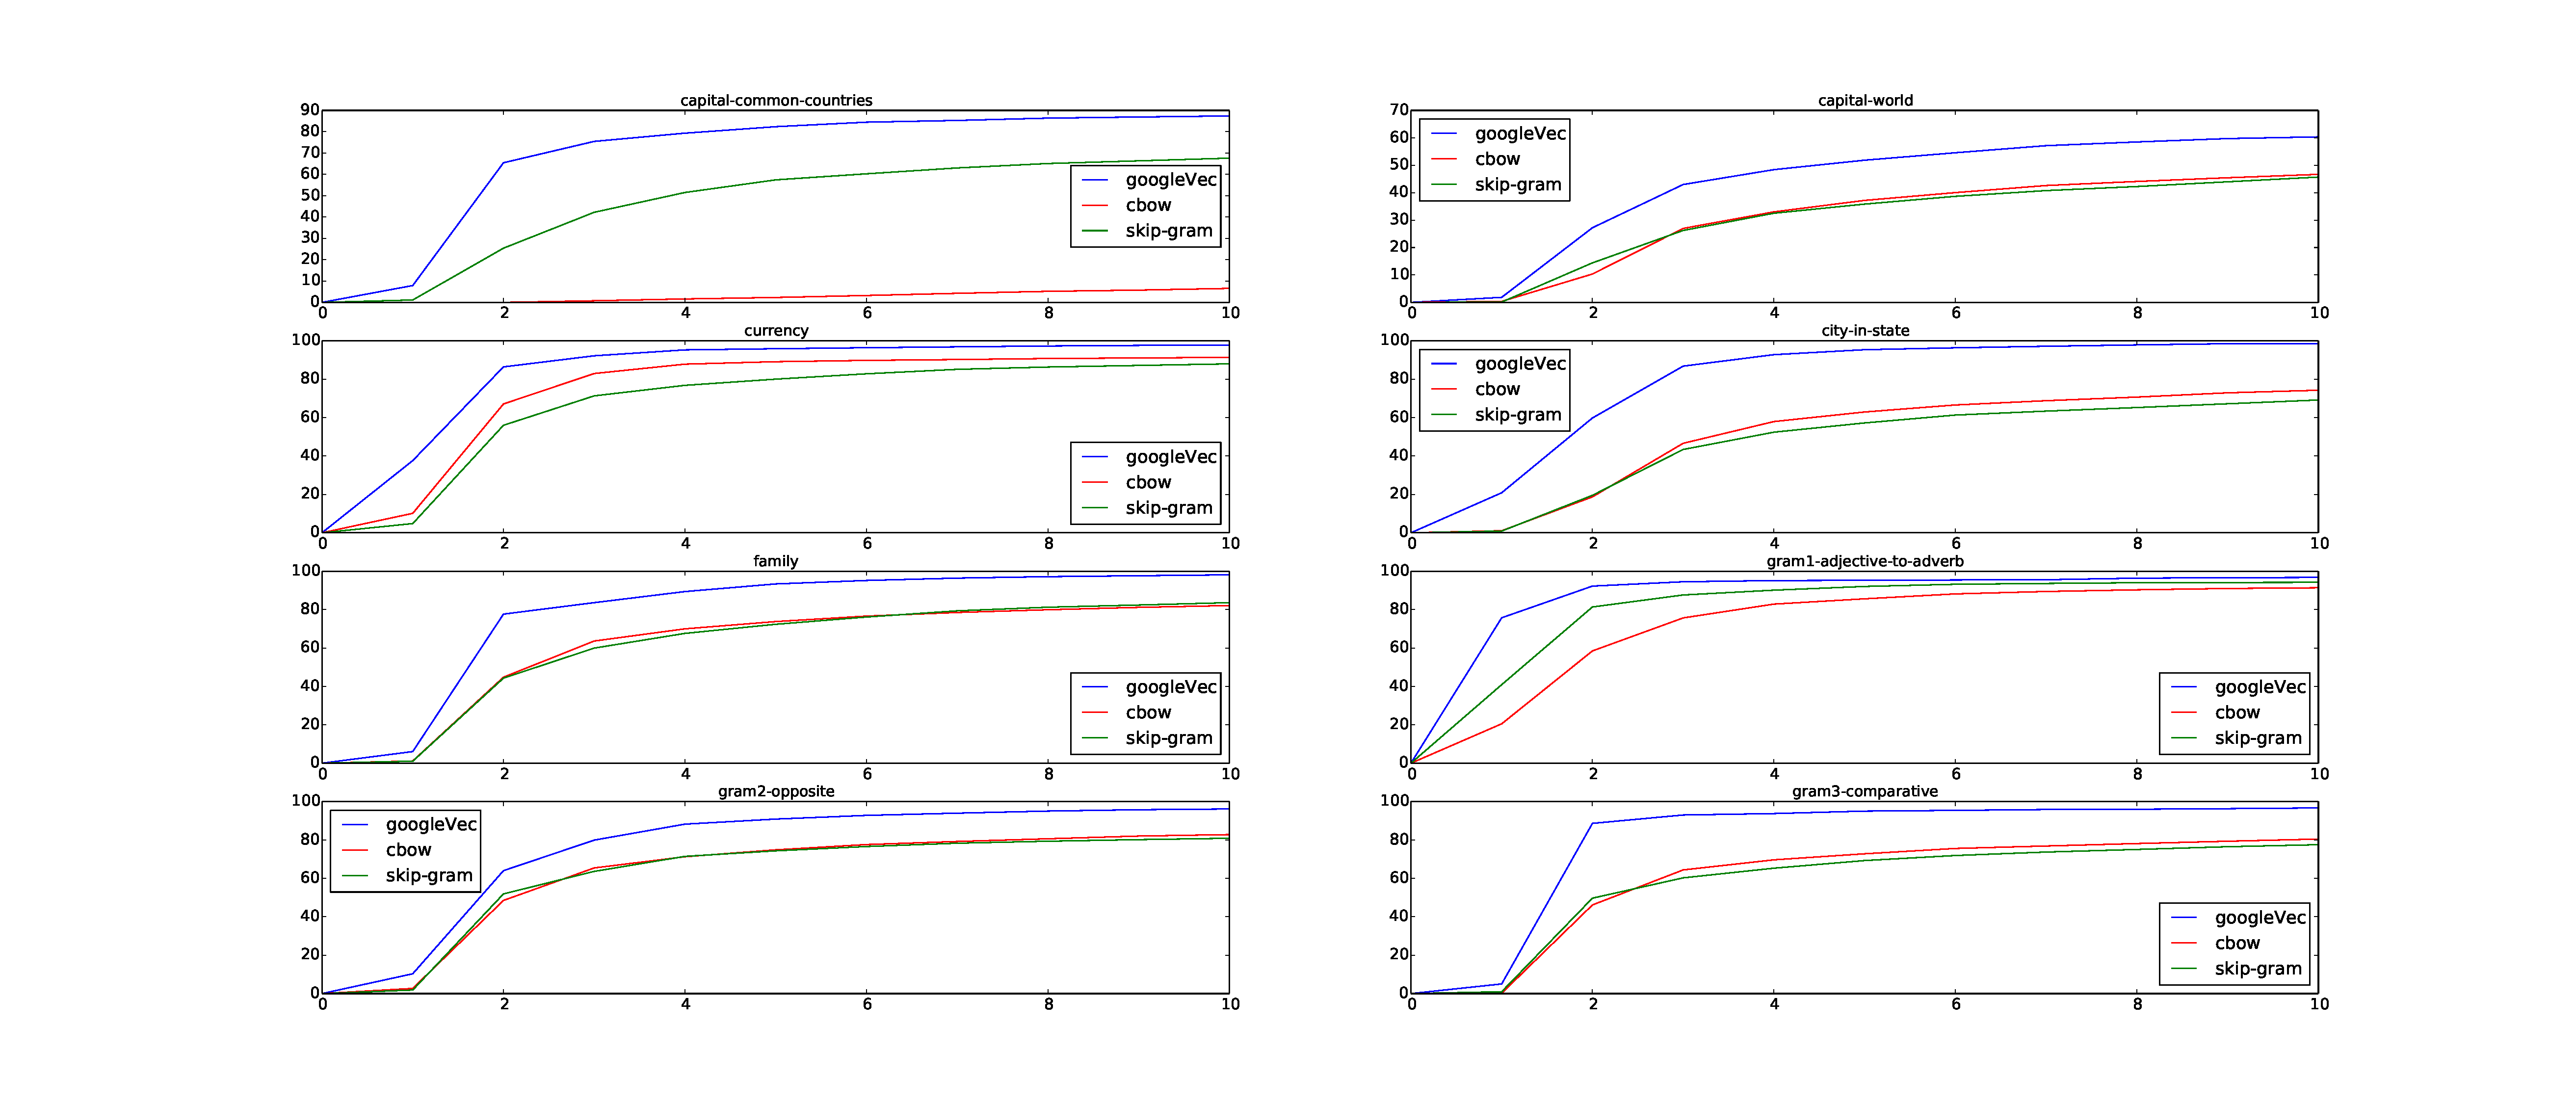
\includegraphics[width=\textwidth]{./images/top_k.pdf}
\caption{Top K accuracy for increasing K.}
\label{fig:top_k}
\end{figure}

\begin{figure}[h]
\centering
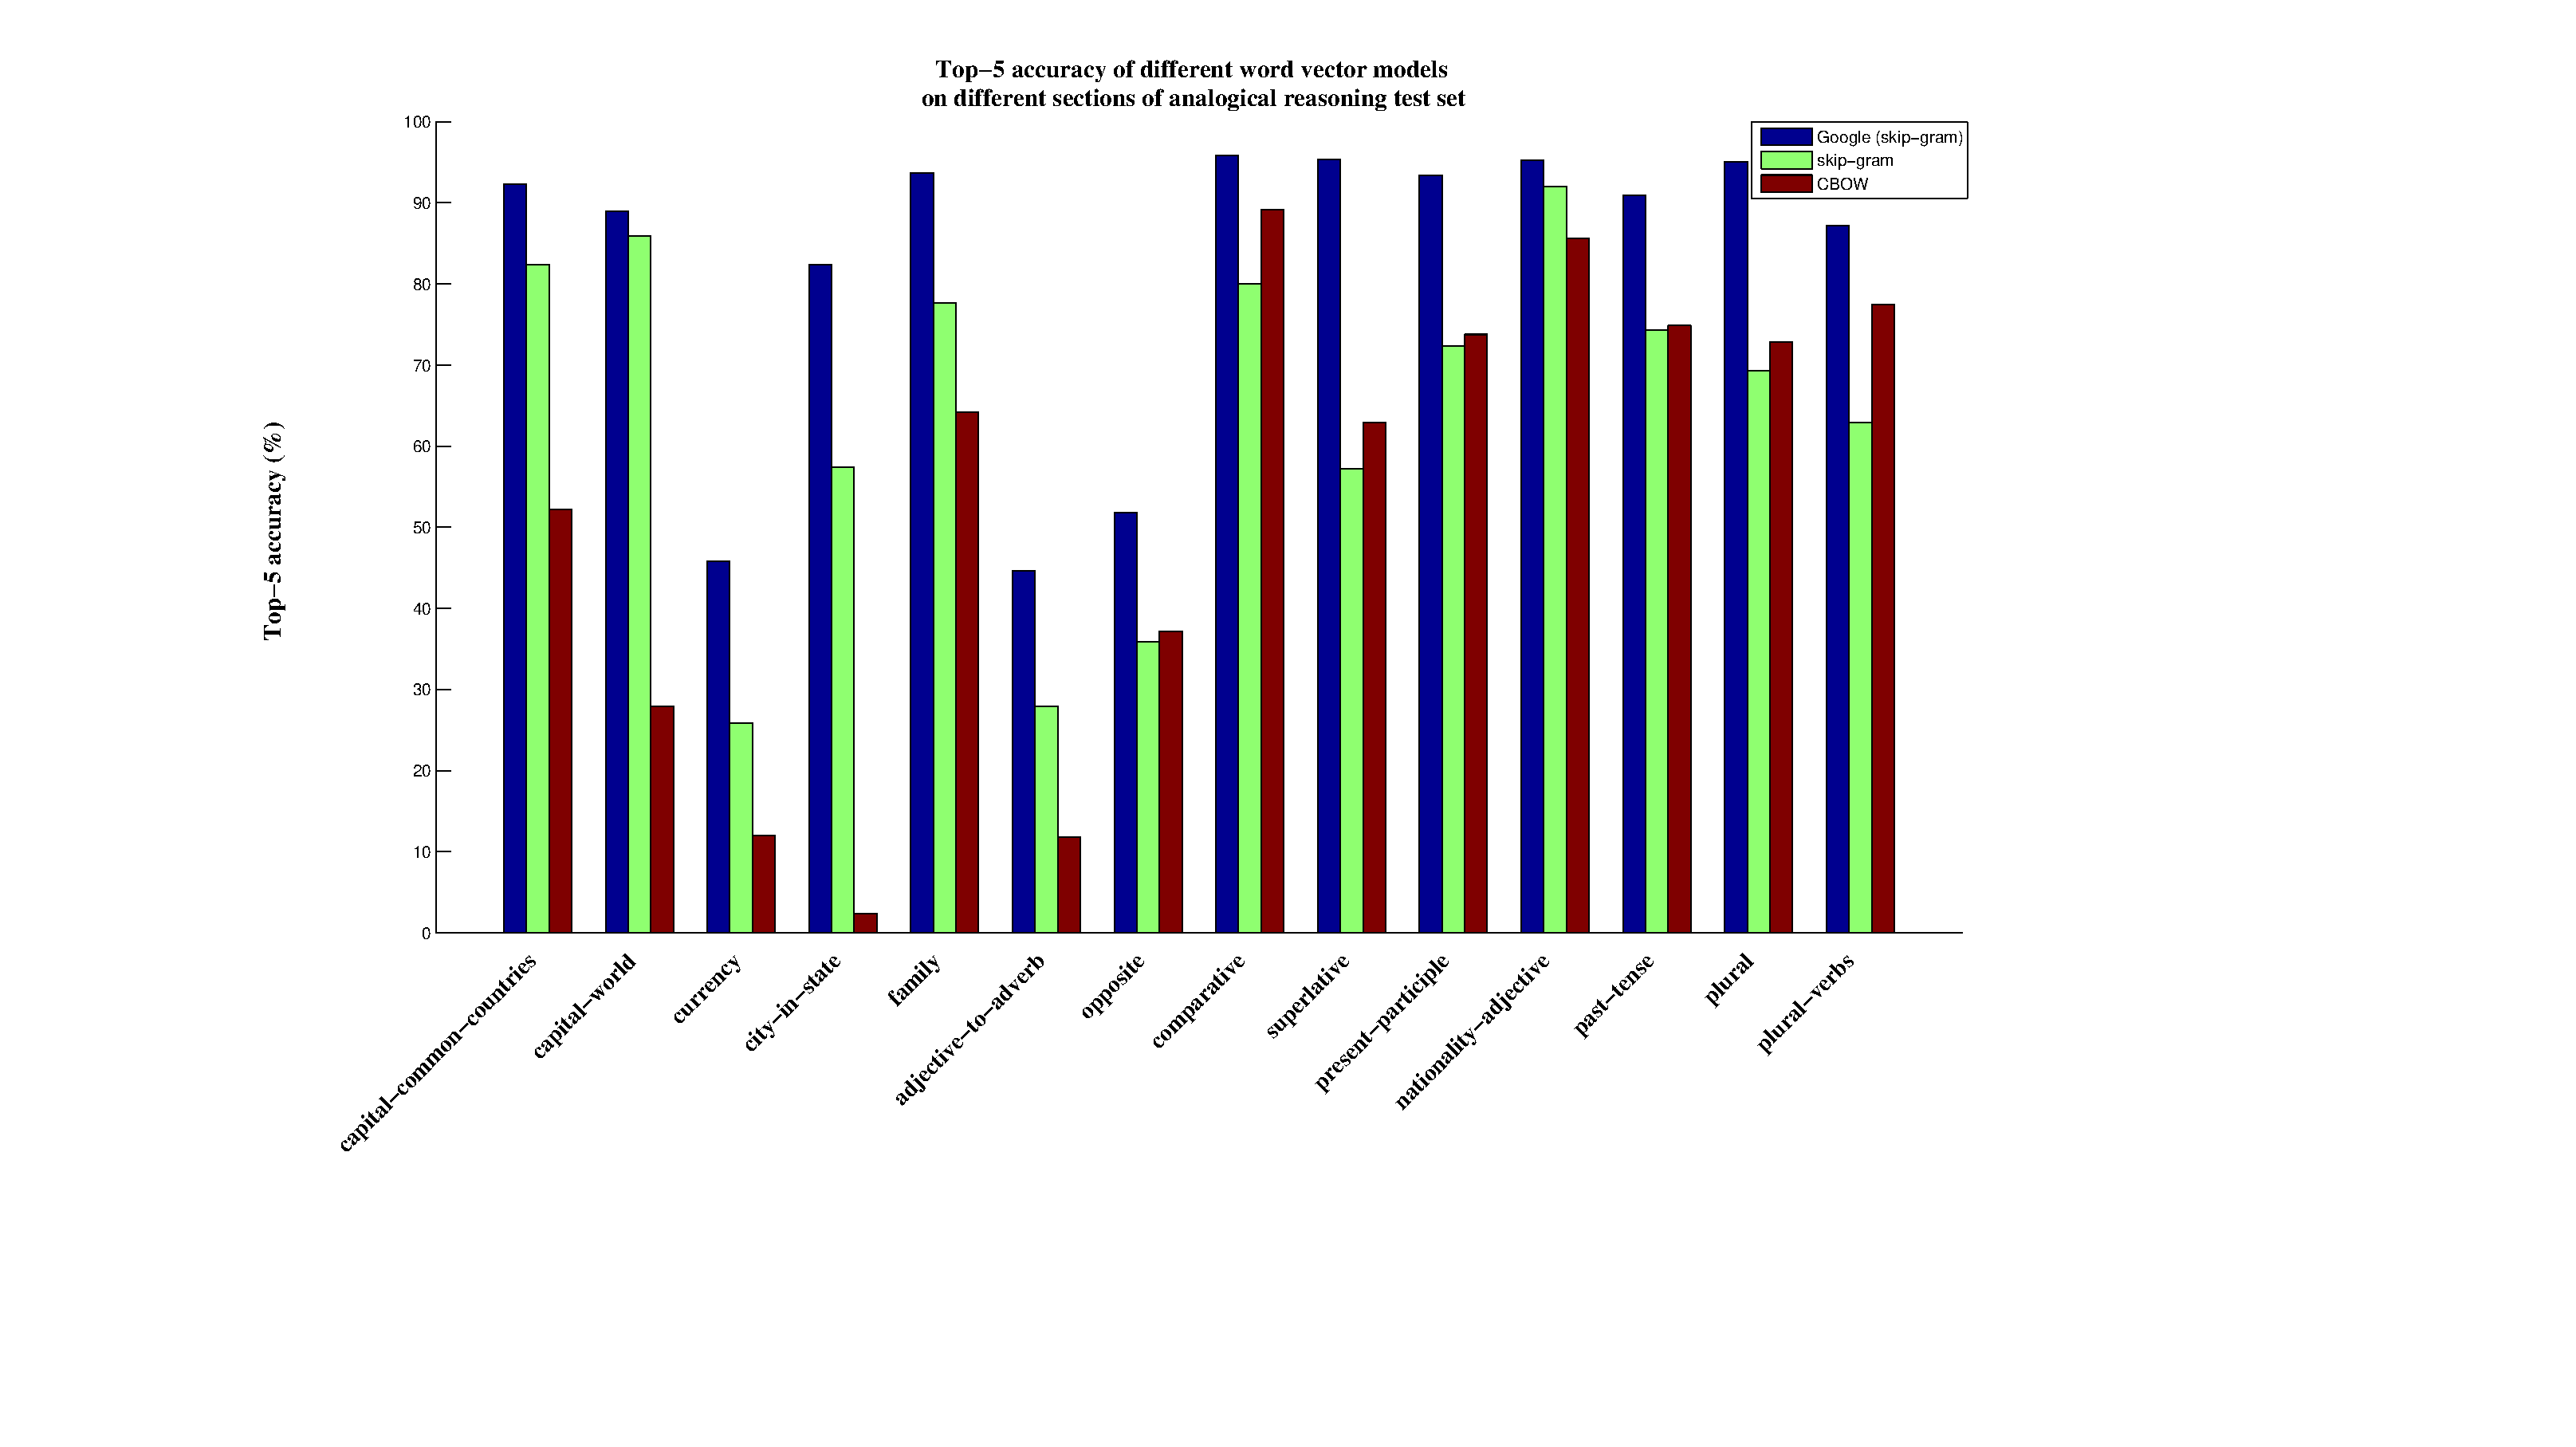
\includegraphics[width=\textwidth]{./images/analog_accuracy_per_question.eps}
\caption{Top-5 accuracy per analogy question type.}
\label{fig:accuracy_per_question}
\end{figure}


\subsubsection{Visualizing low dimensional approximations of embedding space}

We explored the low dimensional structure of different words used in the analogical reasoning set. In an attempt to gain some insight into the embedding space we did the following:
\begin{enumerate}
  \item Take 3 words from one of the quartets in the analogical reasoning test set and compute the subspace that best fits the corresponding word vectors. (For example, fine the plane that best approximates $\phi(Paris), \phi(France)$ and $\phi(London)$. 
  \item Project all word vectors onto this plane.
  \item Throw away all vectors greater than some threshold away from the plane (in the examples plotted below we kept only the closest 20 vectors).
  \item Plot the remaining word vectors projected onto the plane, coded based on Euclidean distance from the plane (the radius of the point is proportional to the distance, so larger implies farther away). 
  \item Highlight points that would be predicted (using the projected vectors) within the top $k$ (we used $k = 5$) using the vector offset method.
\end{enumerate}


\begin{figure}[t]
\centering
\subfigure[Greece : Athens - Thailand : Bangkok]{
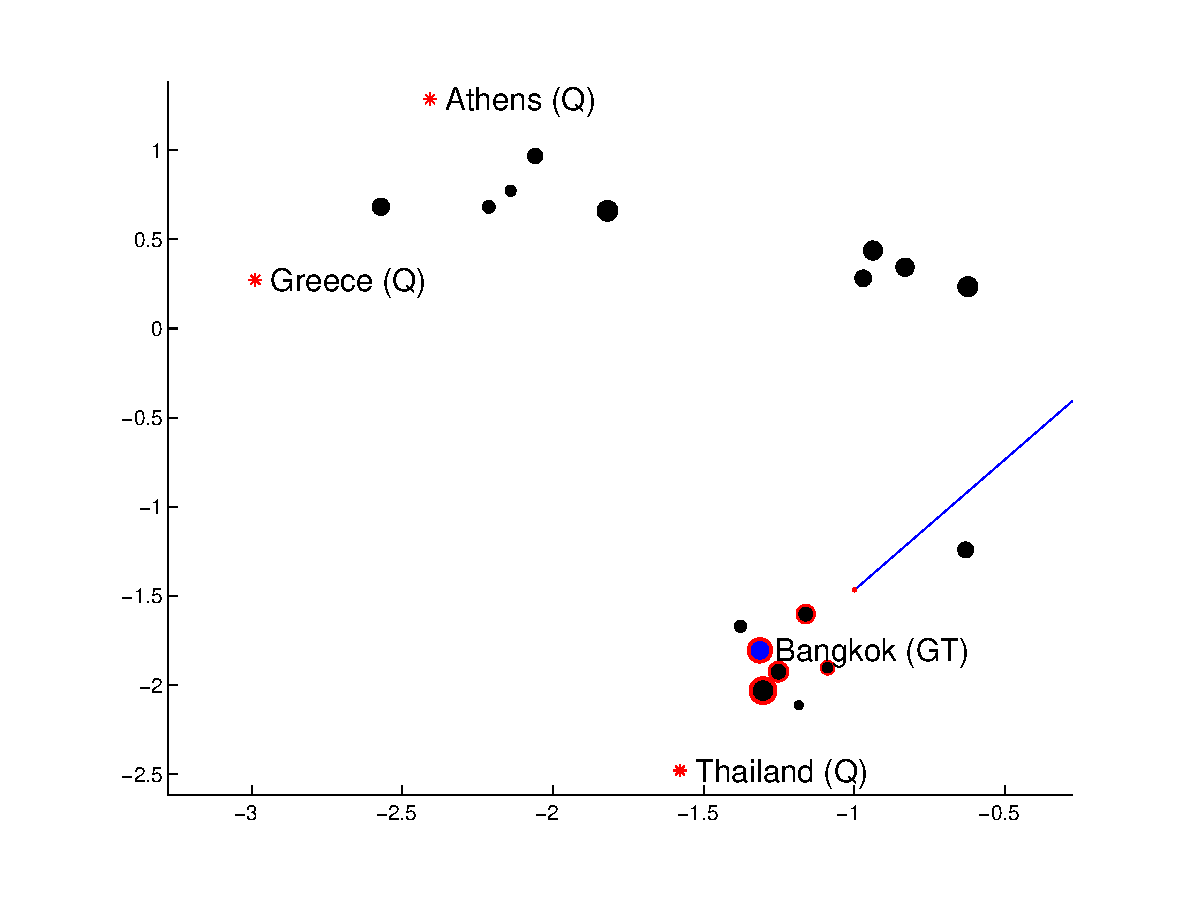
\includegraphics[width=.45\textwidth]{./images/greece_athens_thailand_bangkok.eps}
}
\subfigure[Greece : Athens - Japan : Tokyo]{
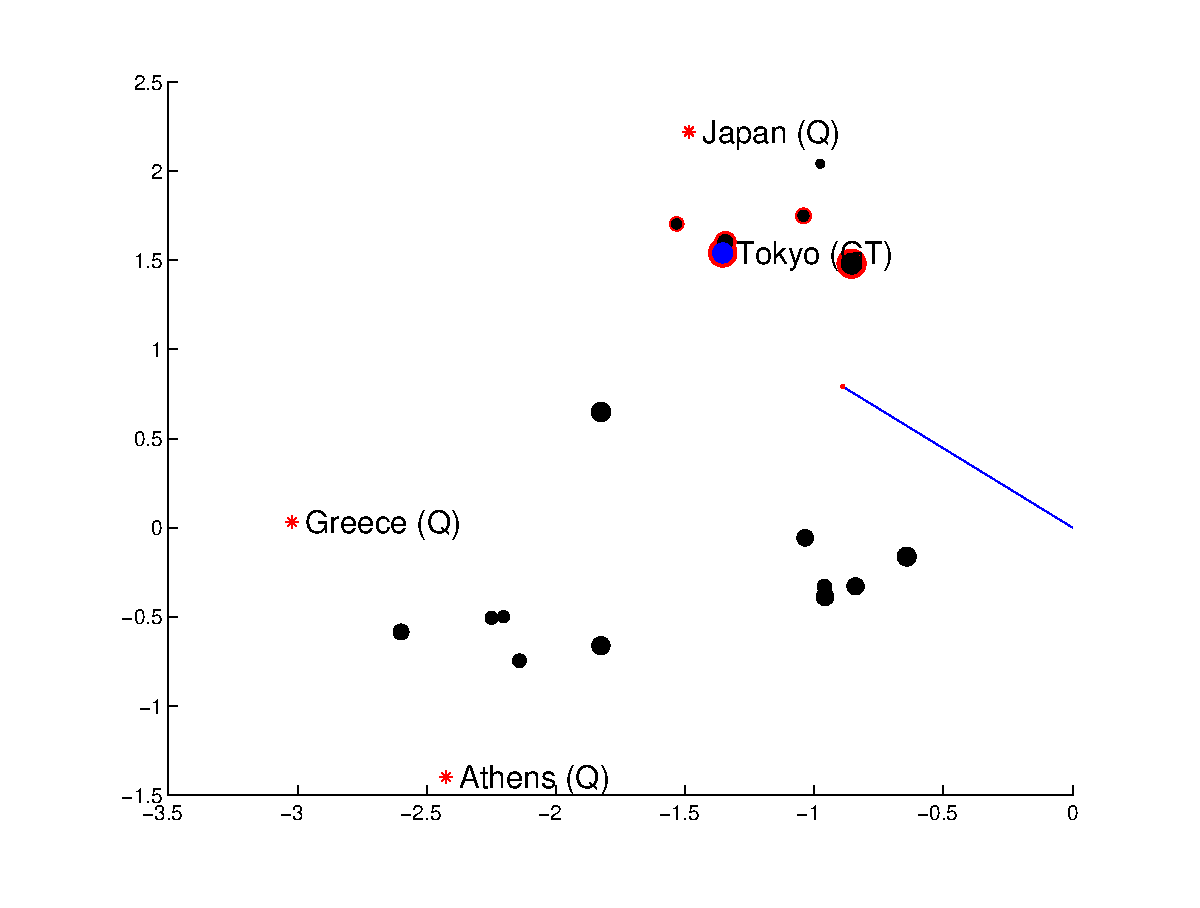
\includegraphics[width=.45\textwidth]{./images/greece_athens_japan_tokyo.eps}
}

\subfigure[Greece : Athens - Russia : Moscow]{
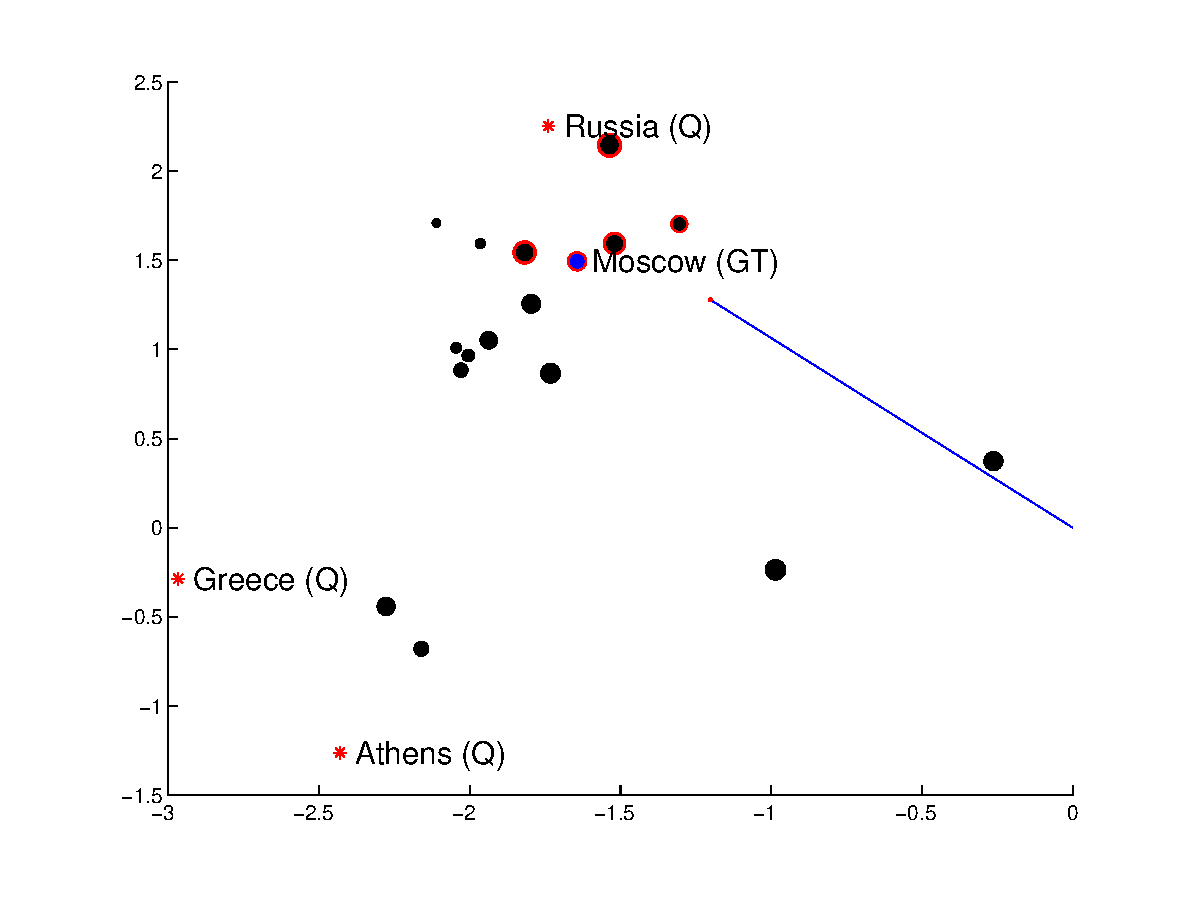
\includegraphics[width=.45\textwidth]{./images/greece_athens_russia_moscow.eps}
}
\subfigure[Greece : Athens - Egypt : Cairo]{
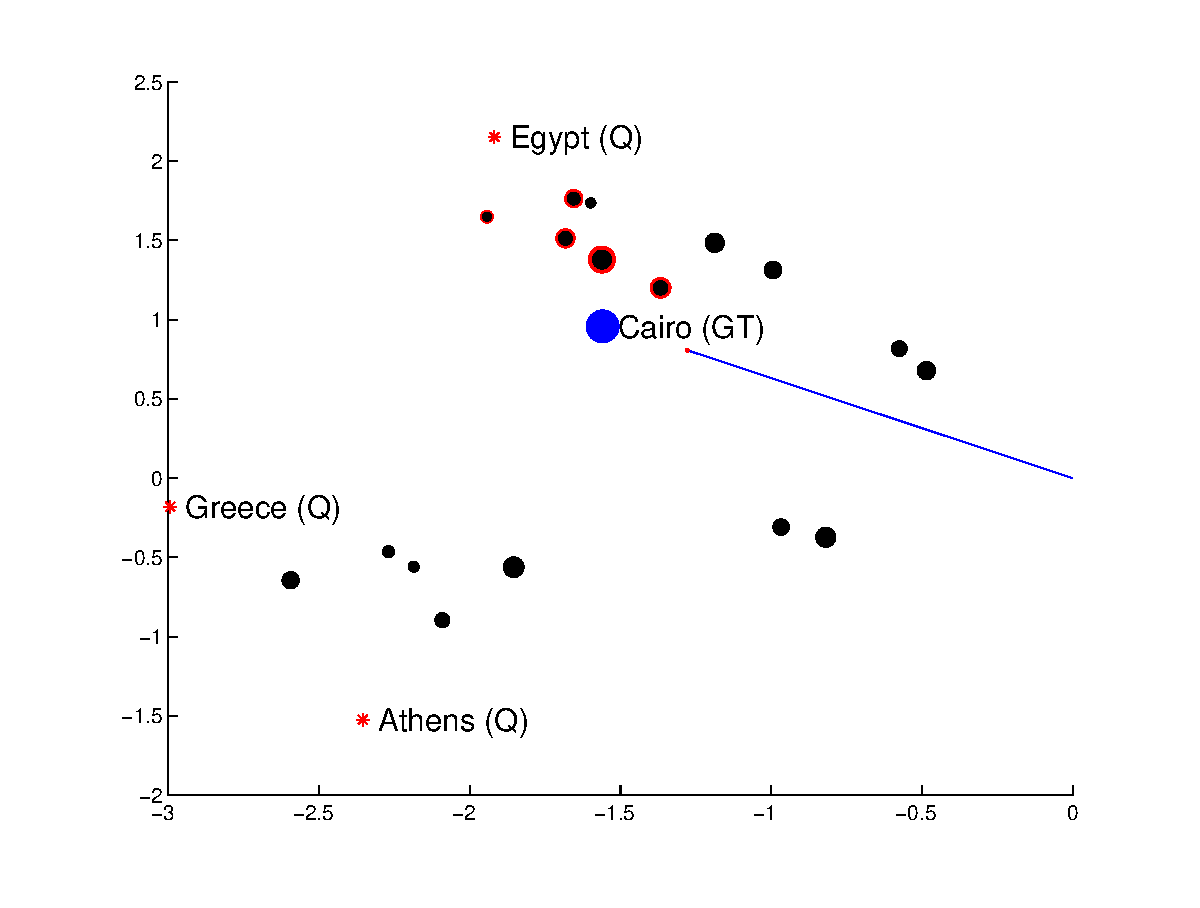
\includegraphics[width=.45\textwidth]{./images/greece_athens_egypt_cairo.eps}
}
\caption{Analogical reasoning word vectors projected onto 2D plane}
\label{fig:offsetProj}
\end{figure}

Figure \ref{fig:offsetProj} shows for of these such plots using country-capital analogies. In the plots, the red $*$'s denote the analogical query vectors, $\phi(A), \phi(B), \phi(C)$, projected onto the plane of best fit. The red $\cdot$ denotes the vector computed with the vector offset method ($\phi(B) - \phi(A) + \phi(C)$) projected onto the same plane. A blue line is drawn format he origin to this point to elucidate the direction of the vector (recall we only care about the direction of the vector, not it's magnitude). The true solution vector, $\phi(D)$, projected onto the same plane, is plotted with a blue circle. The radius of the circle indicates the distance the point lies form the plane. Finally, the black points denote the 20 closest word vectors to the plane, where again, the size of the point indicates distance front he plane. The points that would be predicted as being in the top-5 solution set are highlighted in red. Figure \ref{fig:offsetProj} (a)-(c) are examples where the correct answer is found int he top-5 (as indicated by the red circle around the blue point). Figure \ref{fig:offsetProj} (d) shows an examples where the correct word is not found in the top-5 set. This case is interesting because the true solution is very close (based on cosine distance) to ($\phi(B) - \phi(A) + \phi(C)$), however it was too far away from the plane to be found. 

One could imagine constructing a new method of answering the analogical query questions using this information by first restricting the set of possible solution vectors to only the $p$ closest ones to the plane and then doing the top-$k$ search for a solution. We tried this experiment for a variety of $k$ and $p$ and did not find it to perform better than the original method. This is to be expected given the huge amount of information that is being thrown away. However, it is interesting that the method does allow some questions to be answered correctly. We achieved a 30\% top-5 accuracy for $p = 20$, which means that a significant amount of information is retained after projecting down into 2 dimensions.  

\subsubsection{Finding analogical relations}

Our final goal was to try and uncover analogical relation automatically. First we generated some visualizations to help guide our work. Figure \ref{fig:2D_offsets} plots vector offsets for capital-country word pairs projected onto 2D. This image was generated by first selected all the word vectors that are either a country name or a capital of a country. We then computed the offset vectors for every possible pair. There are four different type of offsets:
\begin{enumerate}
\item capital - country ( A subset of these will be true (capital, country) relations such as $Paris - France$ and $London - England$. Another, much larger, subset will consist of the remaining capital country pairs such as $Paris - Thailand$ and $Athens - London$.)
\item country - capital ( A subset of these will be true (country, capital) relations such as $France - Paris$ and $England - London$. Another, much larger, subset will consist of the remaining (country, capital) pairs such as $Thailand - Paris$ and $London - Athens$.)
\item country - country
\item capital - capital
\end{enumerate}

We then computed the SVD decomposition of the matrix of offsets and projected them all down to 2 dimensions. The points in Figure \ref{fig:2D_offsets} are color/shape coded based on what kind of offset they are (type 1-4 above). The circles (upper right diagonal cluster) correspond to $capital - country$ offsets. The crosses (lower cluster diagonal blob) correspond to $country - capital$ offsets. The stars and dots (middle cluster) correspond to $capital - capital$ and $country - country$ offsets respectively. Finally, the red points are $country - capital$ or $capital - country$ offsets that correspond to true capital/country relationships. In other words, all the red circles are analogous tone another and all of the red crosses are analogous to one another. Ideally, we would like to be able to separate  the red points form the rest. The image shows that there is a significant amount of structure, even in 2 dimensions, which suggests that we should be able to automatically discover which offsets correspond to true analogies. Figure \ref{fig:3D_offsets} shows only the $capital - country$ offsets (true and incorrect relations) projected into 3 dimensions. The figure shows that the true (red) and incorrect (blue) relations can begin to be disambiguated in 3 dimensions. 

\begin{figure}[h]
\centering
\includegraphics[width=\textwidth]{./images/capital_country_2D_proj.eps}
\caption{All combinations of vector offsets for country and capital words projected onto 2 dimensions.}
\label{fig:2D_offsets}
\end{figure}

\begin{figure}[h]
\centering
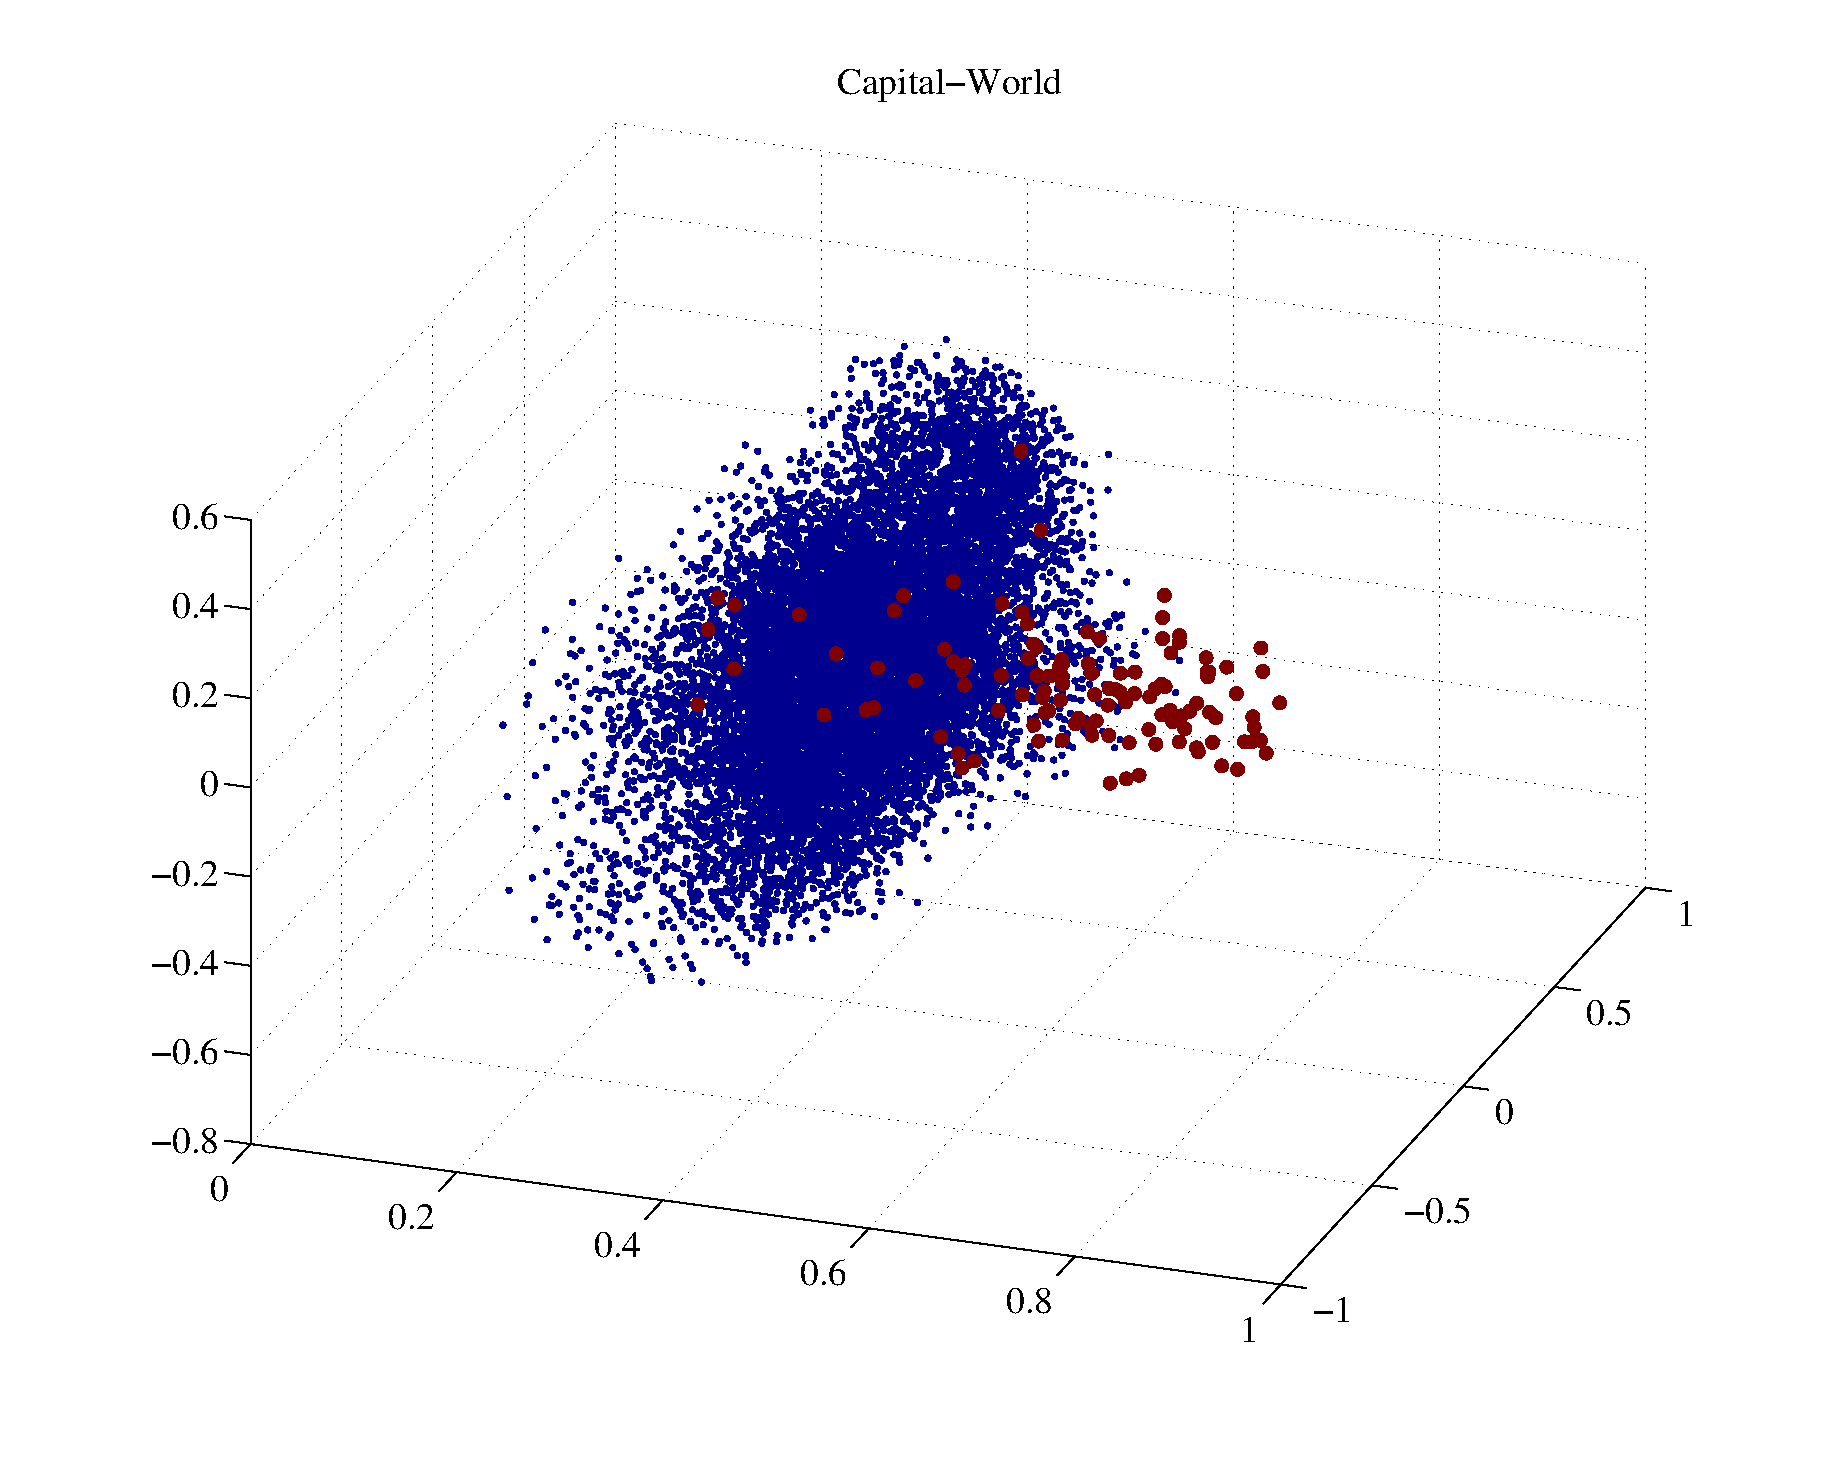
\includegraphics[width=\textwidth]{./images/capital_world.eps}
\caption{All capital - country offsets projected onto 3 dimensions. }
\label{fig:3D_offsets}
\end{figure}

Our approach to discovering analogical relations is based on the basic insight that the cosine distance for pairs of offsets will be small if the pairs are analogous. In other words we would expect 
\begin{align*}1 - \frac{(\phi(brother) - \phi(sister)) \cdot (\phi(father) - \phi(mother))}{ \| \phi(brother) - \phi(sister)) \| \| (\phi(father) - \phi(mother)\|}\end{align*}
while we would expect 
 \begin{align*}1 - \frac{(\phi(cat) - \phi(sister)) \cdot (\phi(running) - \phi(Canada))}{ \| \phi(cat) - \phi(sister)) \| \| (\phi(running) - \phi(Canada)\|}\end{align*} 
 to be large. 

We attempted to cluster word vector offsets based on cosine distance.We tried two methods: (1) Spectral clustering where the cosine distance between offsets is used as the affinity matrix (2) K-means there cosine distance is used as the distance metric. 

Table \ref{tab:analogies1} shows examples of pairs from clusters found when the clustering is done on a large set of word vectors containing 50,000 common words. The pairs that appear in a given cluster are analogous to one another, but in a very uninteresting way. The clusters tend to contains words such as $the, in, that, for,$ etc. as one of the words in the offsets pairs and the other words form a particular category. We hypothesize that this is because words such as $in, the, the,$ etc. all have very similar vector representations. Although, the clusters found here do make sense, they are uninteresting form an analogy discovery perspective. 

Our next experiment tried to address this problem by restricted the set of word vectors we sued to compute the offsets to those words that are either countries, capitals of countries, currency of countries, states or state capitals. In this case we did find some clusters with true analogies. Examples format hess clusters are shown in table \ref{tab:analogies2}. Other clusters, not shown in the table tended to have reasonable elements, but not interesting analogies. For example, one of the clusters found consisted of eastern European countries paired with South American countries. 

Finally, we performed another clustering experiment using only the terms front he "family" section of the analogical reasoning set. This section consists of pairs such as $(brother, sister), (mother, father), $etc. We used all possible pairings to compute offsets. Examples from a selection of the resulting clusters is shown in table \ref{tab:analogies3}. The third cluster in the table corresponds to the analogies outlined in the analogical reasoning set. The other clusters also correspond to interesting analogical relations. 

We can conclude from these results that it is possible to uncover interesting analogical relations using very simple cluster methods. It is important to restrict the set of words in some manner so as not to have very common words that have similar representations (such as $and, the, for, in, that$, etc.) pair with other broad categories. While these "analogous pairs" make sense, they are uninteresting. 

\begin{table}[h]
	\caption{Analogies found with no restriction on word vector set.}
	\label{tab:analogies1}
	\centering
    \begin{tabular}{| c | c | c | c |}
    \hline
    \textbf{Cluster 1} & \textbf{Cluster 2} & \textbf{Cluster 3} & \textbf{Cluster 4}\\ \hline
    mother - in & in - dog & in - Thai & that - stood \\
    \hline
    daughter - in & in - cat & in - Myanmar & that - jumped\\
    \hline
    grandmother - in & in -  rabbit & in - Zambian & that - slipped\\
    \hline
    granddaughter - in & in - turtle & for - Ugandan & the - dropped \\
    \hline
    mother - for & for  - bird & for - Cambodian & the - stood \\
    \hline
    niece - for & for - squirrel & that - Thai & the - jumped\\
    \hline
    \end{tabular}
\end{table}


\begin{table}[h]
	\caption{Analogies found with subset of word vector set.}
	\label{tab:analogies2}
	\centering
    \begin{tabular}{| c | c |}
    \hline
    \textbf{Currency / Country terms} & \textbf{Country / Capital terms} \\ \hline
    rupee - India & Russia - Moscow\\
   \hline
    zloty - Poland & Romania - Bucharest \\
   \hline
    ruble - Russia & Croatia - Zagreb\\
   \hline
    ringgit - Malaysia & Hungary - Budapest\\
   \hline
    hryvnia - Ukraine & Venezuela - Caracus\\
   \hline forint - Hungary & Ukraine - Kiev\\
    peso - Mexico & Thailand - Bangkok\\
    \hline
    \end{tabular}
\end{table}

\begin{table}[h]
	\caption{Analogies found with subset of word vector set containing family relations and male/female pronouns.}
	\label{tab:analogies3}
	\centering
    \begin{tabular}{| c | c | c | c |}
    \hline
    \textbf{M/F different generations} & \textbf{M/F royalty terms} & \textbf{M/F complementary terms} & \textbf{M/F pronouns}\\ \hline
	niece - grandma & princess - mother & daughter - son & his - son\\
	\hline
	daughter - grandma & princess - daughter & mother - father & her - daughter\\
	\hline
	nephew - grandpa & queen - mother & nice - nephew  & his - father \\
	\hline
	son - dad & prince - son & aunt - uncle &her - mother \\
	\hline
	son - grandpa & prince - father & sisters - brothers & her - niece\\
	\hline
	daughter - mom & queen - granddaughter & sister - brother & she - mother\\
    \hline
    \end{tabular}
\end{table}


